\def\name {Sofya Yanovskaya}
\documentclass{scrartcl}
\usepackage[landscape]{geometry}
\usepackage{chancery}
\usepackage{anyfontsize}
%\newfont{\hge}{hge scaled 5000}
\usepackage{yfonts}
\usepackage[utf8]{inputenc} 
\usepackage[T1]{fontenc} 
\usepackage[dvipsnames]{xcolor} 
\usepackage[object=vectorian]{pgfornament}
\usetikzlibrary{calc}
\pagestyle{empty}
\oddsidemargin -1.2cm
\textwidth 25.8cm
\topmargin -2.8cm
\textheight 19.8cm
\begin{document}
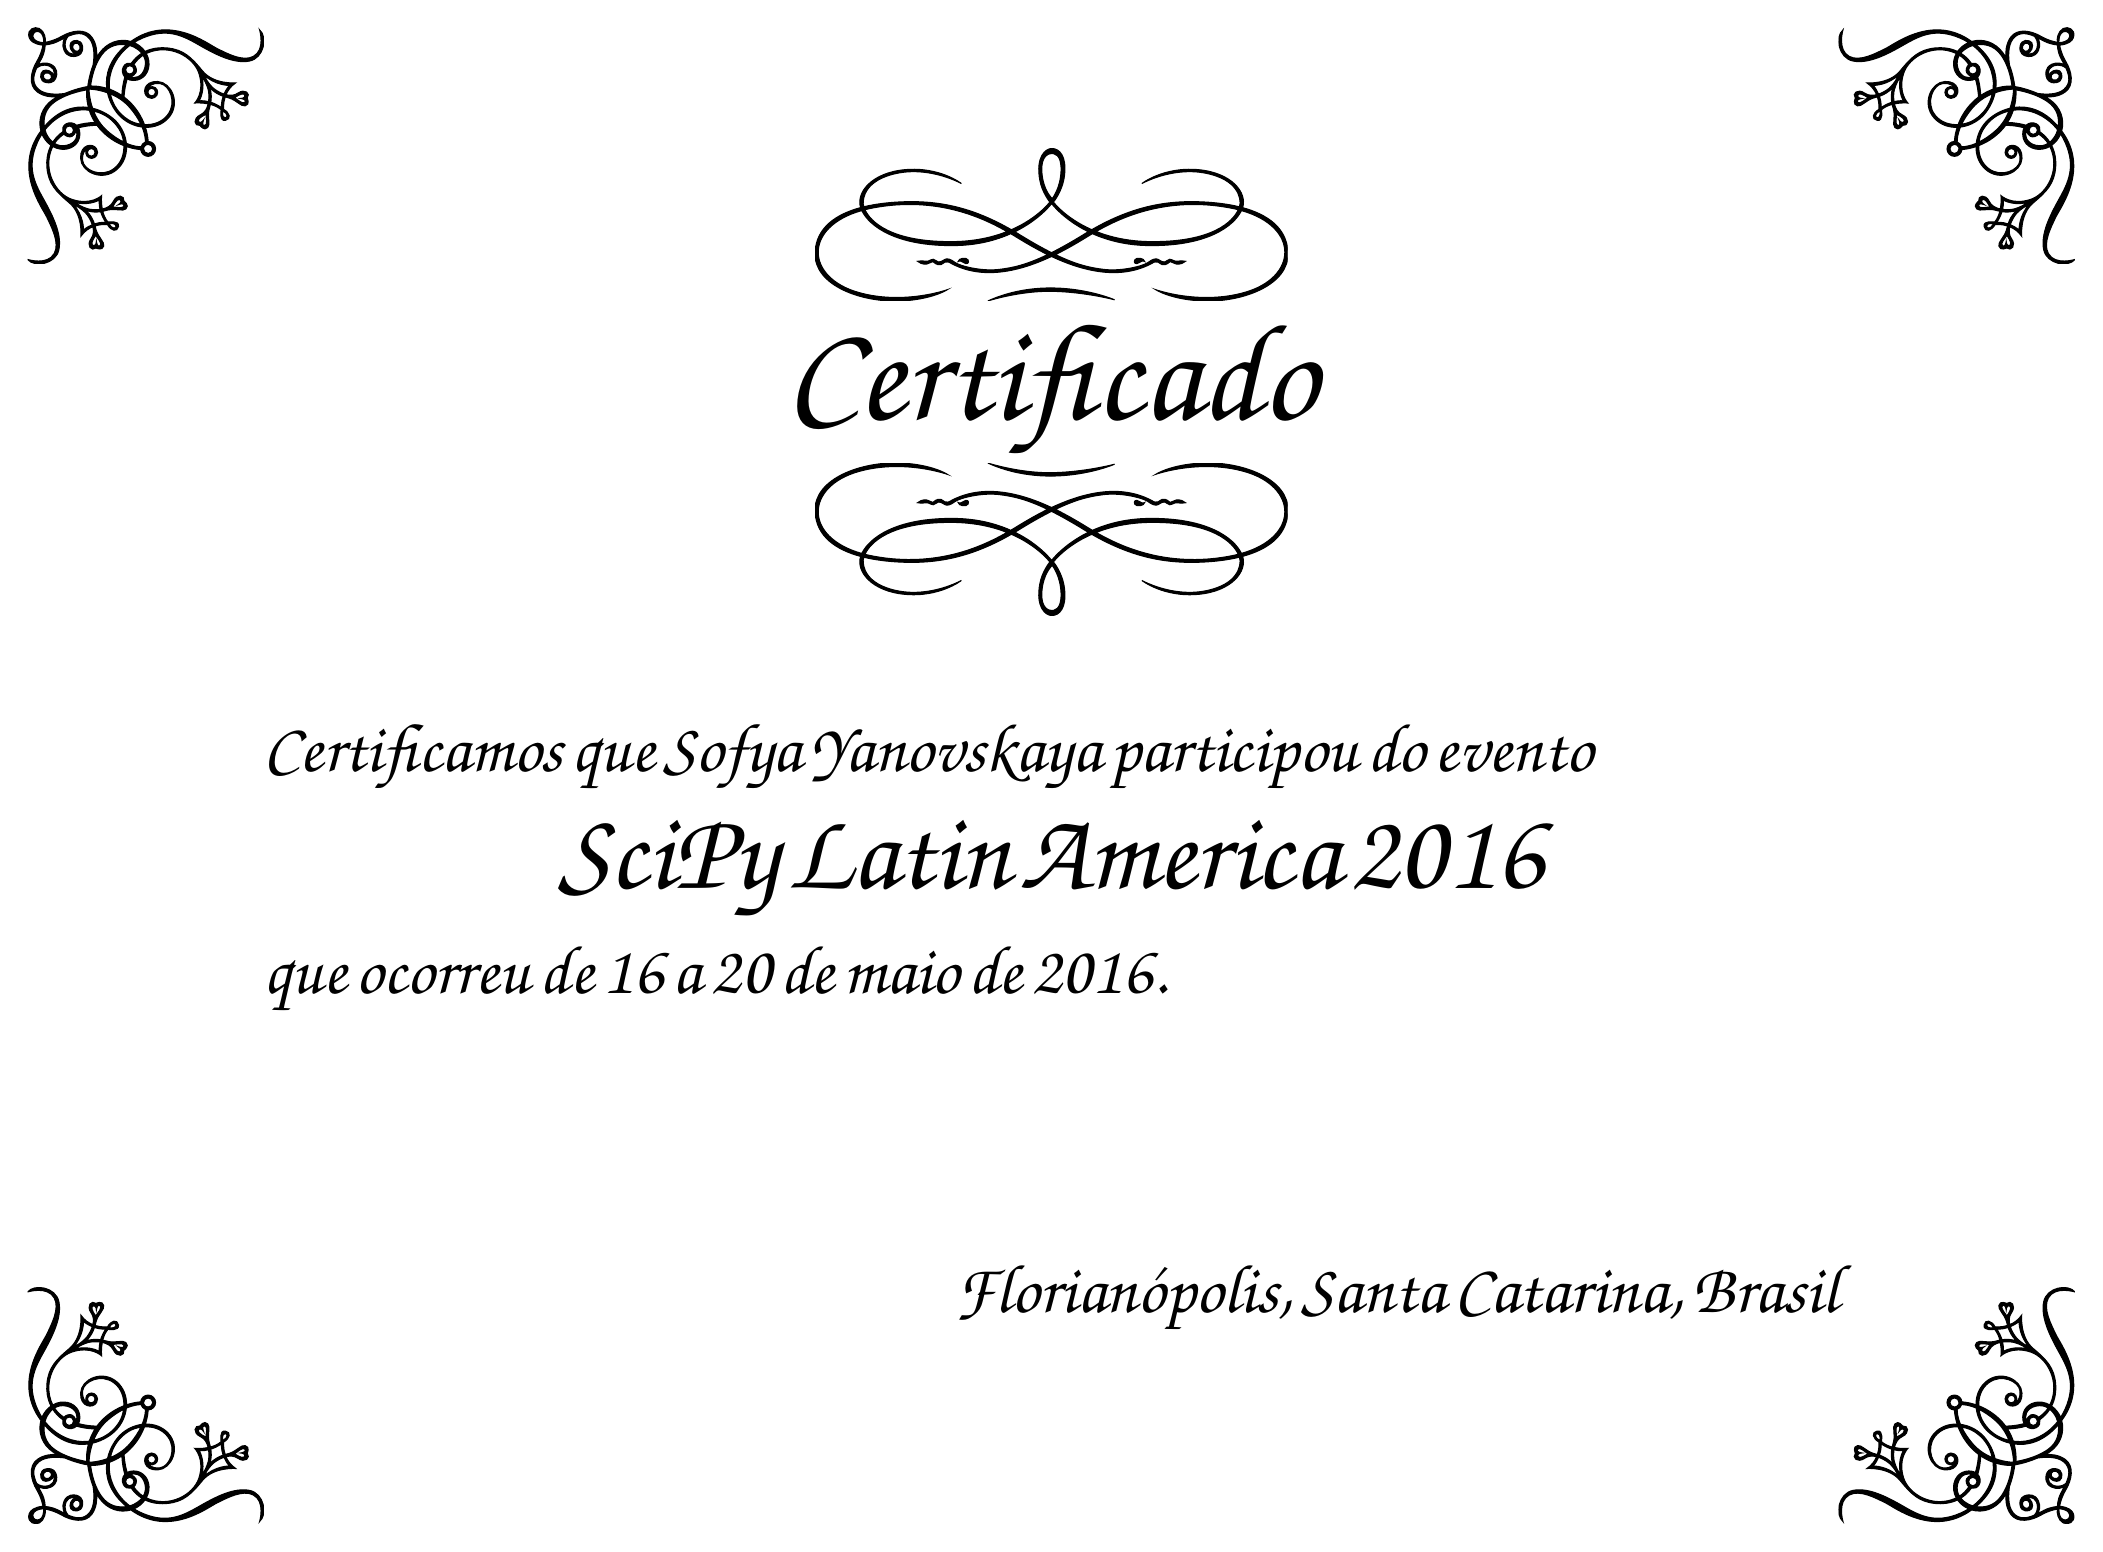
\begin{tikzpicture}[every node/.style={inner sep=0pt}]   
   %\draw[help lines] grid (26,19);
   \node (CNW) at (1.5,17.5) {\pgfornament[width=3cm]{61}};
   \node (CNE) at (24.5,17.5) {\pgfornament[width=3cm,symmetry=v]{61}}; 
   \node (CSW) at (1.5,1.5) {\pgfornament[width=3cm,symmetry=h]{61}}; 
   \node (CSE) at (24.5,1.5) {\pgfornament[width=3cm,symmetry=c]{61}};
   \node [text width=20cm] at (13,9)
      {
         \begin{center}
            {\fontsize{50}{60}\selectfont Certificado}
         \end{center}
         \vskip3cm
         \Huge{
            Certificamos que 
            \name\
            participou do evento}
          \begin{center}
            {\fontsize{40}{50}\selectfont SciPy Latin America 2016}
         \end{center}
         \Huge{que ocorreu de 16 a 20 de maio de 2016.}
         \vskip3cm
         \begin{flushright}
            Florianópolis, Santa Catarina, Brasil
         \end{flushright}
      };
   \node at (13,16.5) {\pgfornament[width=6cm,symmetry=h]{75}};
   \node at (13,12.5) {\pgfornament[width=6cm]{75}};
\end{tikzpicture}
\end{document}











































































































































































































































































































































































































































































